\documentclass{article}
% numbered citations [1], [2,3]; the reference list follows order of first citation
\PassOptionsToPackage{numbers,sort&compress}{natbib}
\usepackage[preprint]{neurips_2026}

\usepackage[utf8]{inputenc}
\usepackage[T1]{fontenc}
\usepackage{hyperref}
\hypersetup{hidelinks} % links stay clickable, without coloured boxes around citation numbers
\usepackage{url}
\usepackage{booktabs}
\usepackage{amsfonts}
\usepackage{amsmath}
\usepackage{amssymb}
\usepackage{microtype}
\usepackage{xcolor}
\usepackage{graphicx}

% This is an ES 678 course paper, not a conference submission.
\makeatletter
\renewcommand{\@noticestring}{ES 678 Course Project}
\makeatother
\graphicspath{{../results/figures/}}
\let\realincludegraphics\includegraphics
\renewcommand{\includegraphics}[2][]{\IfFileExists{../results/figures/#2}{\realincludegraphics[#1]{#2}}{\fbox{\parbox[c][3cm][c]{.4\linewidth}{\centering\small missing: \detokenize{#2}}}}}
% Auto-generated by scripts/paper_numbers.py. Do not edit by hand.
\newcommand{\AccCHun}{71.0}
\newcommand{\AccCTen}{92.3}
\newcommand{\AccCTenR}{92.4}
\newcommand{\AccINet}{78.4}
\newcommand{\AccMNIST}{99.1}
\newcommand{\AciCHunAciAll}{89.7}
\newcommand{\AciCHunAciCov}{90.0}
\newcommand{\AciCHunAciSize}{88.8}
\newcommand{\AciCHunFixAll}{60.8}
\newcommand{\AciCHunFixCov}{11.6}
\newcommand{\AciCHunFixSize}{8.5}
\newcommand{\AciCTenAciAll}{89.7}
\newcommand{\AciCTenAciCov}{90.0}
\newcommand{\AciCTenAciSize}{7.4}
\newcommand{\AciCTenFixAll}{68.5}
\newcommand{\AciCTenFixCov}{44.4}
\newcommand{\AciCTenFixSize}{2.2}
\newcommand{\AciCTenRAciAll}{89.8}
\newcommand{\AciCTenRAciCov}{89.8}
\newcommand{\AciCTenRAciSize}{4.6}
\newcommand{\AciCTenRFixAll}{81.2}
\newcommand{\AciCTenRFixCov}{70.8}
\newcommand{\AciCTenRFixSize}{2.3}
\newcommand{\AciINetAciAll}{\textbf{??}}
\newcommand{\AciINetAciCov}{\textbf{??}}
\newcommand{\AciINetAciSize}{\textbf{??}}
\newcommand{\AciINetFixAll}{\textbf{??}}
\newcommand{\AciINetFixCov}{\textbf{??}}
\newcommand{\AciINetFixSize}{\textbf{??}}
\newcommand{\AciMNISTAciAll}{89.7}
\newcommand{\AciMNISTAciCov}{89.9}
\newcommand{\AciMNISTAciSize}{7.9}
\newcommand{\AciMNISTFixAll}{77.4}
\newcommand{\AciMNISTFixCov}{44.0}
\newcommand{\AciMNISTFixSize}{1.7}
\newcommand{\BelowHundred}{44}
\newcommand{\BsCHunApsVsNaiveS}{2.24}
\newcommand{\BsCHunApsVsNaiveSHi}{2.40}
\newcommand{\BsCHunApsVsNaiveSLo}{2.09}
\newcommand{\BsCHunApsVsNaiveW}{5.7}
\newcommand{\BsCHunApsVsNaiveWHi}{8.3}
\newcommand{\BsCHunApsVsNaiveWLo}{1.0}
\newcommand{\BsCHunClusVsPacS}{-93.27}
\newcommand{\BsCHunClusVsPacSHi}{-91.83}
\newcommand{\BsCHunClusVsPacSLo}{-94.14}
\newcommand{\BsCHunClusVsPacW}{-17.0}
\newcommand{\BsCHunClusVsPacWHi}{-17.7}
\newcommand{\BsCHunClusVsPacWLo}{-23.6}
\newcommand{\BsCHunDistVsNaiveS}{0.01}
\newcommand{\BsCHunDistVsNaiveSHi}{0.02}
\newcommand{\BsCHunDistVsNaiveSLo}{0.00}
\newcommand{\BsCHunDistVsNaiveW}{0.3}
\newcommand{\BsCHunDistVsNaiveWHi}{1.4}
\newcommand{\BsCHunDistVsNaiveWLo}{0.0}
\newcommand{\BsCHunPacVsMondS}{93.62}
\newcommand{\BsCHunPacVsMondSHi}{94.52}
\newcommand{\BsCHunPacVsMondSLo}{92.02}
\newcommand{\BsCHunPacVsMondW}{29.7}
\newcommand{\BsCHunPacVsMondWHi}{37.0}
\newcommand{\BsCHunPacVsMondWLo}{26.7}
\newcommand{\BsCTenApsVsNaiveS}{0.21}
\newcommand{\BsCTenApsVsNaiveSHi}{0.22}
\newcommand{\BsCTenApsVsNaiveSLo}{0.20}
\newcommand{\BsCTenApsVsNaiveW}{9.4}
\newcommand{\BsCTenApsVsNaiveWHi}{9.8}
\newcommand{\BsCTenApsVsNaiveWLo}{7.5}
\newcommand{\BsCTenClusVsPacS}{-0.07}
\newcommand{\BsCTenClusVsPacSHi}{-0.06}
\newcommand{\BsCTenClusVsPacSLo}{-0.07}
\newcommand{\BsCTenClusVsPacW}{-0.9}
\newcommand{\BsCTenClusVsPacWHi}{-0.5}
\newcommand{\BsCTenClusVsPacWLo}{-1.8}
\newcommand{\BsCTenDistVsNaiveS}{0.03}
\newcommand{\BsCTenDistVsNaiveSHi}{0.04}
\newcommand{\BsCTenDistVsNaiveSLo}{0.02}
\newcommand{\BsCTenDistVsNaiveW}{2.1}
\newcommand{\BsCTenDistVsNaiveWHi}{3.0}
\newcommand{\BsCTenDistVsNaiveWLo}{1.0}
\newcommand{\BsCTenPacVsMondS}{0.10}
\newcommand{\BsCTenPacVsMondSHi}{0.10}
\newcommand{\BsCTenPacVsMondSLo}{0.09}
\newcommand{\BsCTenPacVsMondW}{3.3}
\newcommand{\BsCTenPacVsMondWHi}{3.9}
\newcommand{\BsCTenPacVsMondWLo}{2.7}
\newcommand{\BsCTenRApsVsNaiveS}{0.20}
\newcommand{\BsCTenRApsVsNaiveSHi}{0.21}
\newcommand{\BsCTenRApsVsNaiveSLo}{0.19}
\newcommand{\BsCTenRApsVsNaiveW}{10.1}
\newcommand{\BsCTenRApsVsNaiveWHi}{11.0}
\newcommand{\BsCTenRApsVsNaiveWLo}{7.8}
\newcommand{\BsCTenRClusVsPacS}{-0.07}
\newcommand{\BsCTenRClusVsPacSHi}{-0.06}
\newcommand{\BsCTenRClusVsPacSLo}{-0.07}
\newcommand{\BsCTenRClusVsPacW}{-1.0}
\newcommand{\BsCTenRClusVsPacWHi}{-0.4}
\newcommand{\BsCTenRClusVsPacWLo}{-2.0}
\newcommand{\BsCTenRDistVsNaiveS}{0.02}
\newcommand{\BsCTenRDistVsNaiveSHi}{0.05}
\newcommand{\BsCTenRDistVsNaiveSLo}{-0.00}
\newcommand{\BsCTenRDistVsNaiveW}{0.8}
\newcommand{\BsCTenRDistVsNaiveWHi}{2.7}
\newcommand{\BsCTenRDistVsNaiveWLo}{-0.2}
\newcommand{\BsCTenRPacVsMondS}{0.10}
\newcommand{\BsCTenRPacVsMondSHi}{0.10}
\newcommand{\BsCTenRPacVsMondSLo}{0.09}
\newcommand{\BsCTenRPacVsMondW}{3.8}
\newcommand{\BsCTenRPacVsMondWHi}{4.8}
\newcommand{\BsCTenRPacVsMondWLo}{2.7}
\newcommand{\BsINetApsVsNaiveS}{8.51}
\newcommand{\BsINetApsVsNaiveSHi}{8.75}
\newcommand{\BsINetApsVsNaiveSLo}{8.28}
\newcommand{\BsINetApsVsNaiveW}{13.9}
\newcommand{\BsINetApsVsNaiveWHi}{16.8}
\newcommand{\BsINetApsVsNaiveWLo}{4.8}
\newcommand{\BsINetClusVsPacS}{-983}
\newcommand{\BsINetClusVsPacSHi}{-982}
\newcommand{\BsINetClusVsPacSLo}{-983}
\newcommand{\BsINetClusVsPacW}{-39.3}
\newcommand{\BsINetClusVsPacWHi}{-49.6}
\newcommand{\BsINetClusVsPacWLo}{-59.6}
\newcommand{\BsINetDistVsNaiveS}{\textbf{??}}
\newcommand{\BsINetDistVsNaiveSHi}{\textbf{??}}
\newcommand{\BsINetDistVsNaiveSLo}{\textbf{??}}
\newcommand{\BsINetDistVsNaiveW}{\textbf{??}}
\newcommand{\BsINetDistVsNaiveWHi}{\textbf{??}}
\newcommand{\BsINetDistVsNaiveWLo}{\textbf{??}}
\newcommand{\BsINetPacVsMondS}{965}
\newcommand{\BsINetPacVsMondSHi}{966}
\newcommand{\BsINetPacVsMondSLo}{964}
\newcommand{\BsINetPacVsMondW}{52.3}
\newcommand{\BsINetPacVsMondWHi}{69.3}
\newcommand{\BsINetPacVsMondWLo}{59.1}
\newcommand{\BsMNISTApsVsNaiveS}{0.01}
\newcommand{\BsMNISTApsVsNaiveSHi}{0.02}
\newcommand{\BsMNISTApsVsNaiveSLo}{0.01}
\newcommand{\BsMNISTApsVsNaiveW}{5.1}
\newcommand{\BsMNISTApsVsNaiveWHi}{7.4}
\newcommand{\BsMNISTApsVsNaiveWLo}{2.4}
\newcommand{\BsMNISTClusVsPacS}{-0.02}
\newcommand{\BsMNISTClusVsPacSHi}{-0.02}
\newcommand{\BsMNISTClusVsPacSLo}{-0.02}
\newcommand{\BsMNISTClusVsPacW}{-0.9}
\newcommand{\BsMNISTClusVsPacWHi}{-0.5}
\newcommand{\BsMNISTClusVsPacWLo}{-1.5}
\newcommand{\BsMNISTDistVsNaiveS}{0.00}
\newcommand{\BsMNISTDistVsNaiveSHi}{0.00}
\newcommand{\BsMNISTDistVsNaiveSLo}{-0.00}
\newcommand{\BsMNISTDistVsNaiveW}{1.5}
\newcommand{\BsMNISTDistVsNaiveWHi}{3.2}
\newcommand{\BsMNISTDistVsNaiveWLo}{-0.1}
\newcommand{\BsMNISTPacVsMondS}{0.03}
\newcommand{\BsMNISTPacVsMondSHi}{0.03}
\newcommand{\BsMNISTPacVsMondSLo}{0.03}
\newcommand{\BsMNISTPacVsMondW}{2.6}
\newcommand{\BsMNISTPacVsMondWHi}{3.1}
\newcommand{\BsMNISTPacVsMondWLo}{2.4}
\newcommand{\CcCHunAPSTSFive}{\textbf{??}}
\newcommand{\CcCHunAPSTSOne}{\textbf{??}}
\newcommand{\CcCHunNaiveSFive}{\textbf{??}}
\newcommand{\CcCHunNaiveSOne}{\textbf{??}}
\newcommand{\CcCHunTopSFive}{\textbf{??}}
\newcommand{\CcCHunTopSOne}{\textbf{??}}
\newcommand{\CcCTenAPSTSFive}{69.4}
\newcommand{\CcCTenAPSTSOne}{87.1}
\newcommand{\CcCTenNaiveSFive}{43.5}
\newcommand{\CcCTenNaiveSOne}{79.3}
\newcommand{\CcCTenRAPSTSFive}{78.6}
\newcommand{\CcCTenRAPSTSOne}{88.2}
\newcommand{\CcCTenRNaiveSFive}{57.0}
\newcommand{\CcCTenRNaiveSOne}{83.7}
\newcommand{\CcCTenRTopSFive}{64.7}
\newcommand{\CcCTenRTopSOne}{87.5}
\newcommand{\CcCTenTopSFive}{51.3}
\newcommand{\CcCTenTopSOne}{83.9}
\newcommand{\CcINetAPSTSFive}{\textbf{??}}
\newcommand{\CcINetAPSTSOne}{\textbf{??}}
\newcommand{\CcINetNaiveSFive}{\textbf{??}}
\newcommand{\CcINetNaiveSOne}{\textbf{??}}
\newcommand{\CcINetTopSFive}{\textbf{??}}
\newcommand{\CcINetTopSOne}{\textbf{??}}
\newcommand{\CcMNISTAPSTSFive}{\textbf{??}}
\newcommand{\CcMNISTAPSTSOne}{\textbf{??}}
\newcommand{\CcMNISTNaiveSFive}{\textbf{??}}
\newcommand{\CcMNISTNaiveSOne}{\textbf{??}}
\newcommand{\CcMNISTTopSFive}{\textbf{??}}
\newcommand{\CcMNISTTopSOne}{\textbf{??}}
\newcommand{\ChiPCHun}{0.112}
\newcommand{\ChiPCTen}{0.300}
\newcommand{\ChiPCTenR}{0.484}
\newcommand{\ChiPINet}{0.585}
\newcommand{\ChiPMNIST}{0.006}
\newcommand{\ChiRatioCHun}{1.10}
\newcommand{\ChiRatioCTen}{1.07}
\newcommand{\ChiRatioCTenR}{0.99}
\newcommand{\ChiRatioINet}{1.00}
\newcommand{\ChiRatioMNIST}{1.40}
\newcommand{\ClBestMCHun}{100}
\newcommand{\ClBestMCTen}{2}
\newcommand{\ClBestMCTenR}{3}
\newcommand{\ClBestMINet}{\textbf{??}}
\newcommand{\ClBestMMNIST}{3}
\newcommand{\ClBestSizeCHun}{99.41}
\newcommand{\ClBestSizeCTen}{1.18}
\newcommand{\ClBestSizeCTenR}{1.18}
\newcommand{\ClBestSizeINet}{\textbf{??}}
\newcommand{\ClBestSizeMNIST}{0.93}
\newcommand{\ClBestWorstCHun}{99.7}
\newcommand{\ClBestWorstCTen}{88.8}
\newcommand{\ClBestWorstCTenR}{88.8}
\newcommand{\ClBestWorstINet}{\textbf{??}}
\newcommand{\ClBestWorstMNIST}{89.3}
\newcommand{\ClRatioCHun}{1.0}
\newcommand{\ClRatioCTen}{1.1}
\newcommand{\ClRatioCTenR}{1.1}
\newcommand{\ClRatioINet}{\textbf{??}}
\newcommand{\ClRatioMNIST}{1.0}
\newcommand{\CovCHunAPS}{89.5}
\newcommand{\CovCHunAPST}{89.3}
\newcommand{\CovCHunClus}{89.3}
\newcommand{\CovCHunClusPAC}{92.0}
\newcommand{\CovCHunDist}{89.6}
\newcommand{\CovCHunDistAPS}{89.3}
\newcommand{\CovCHunLearned}{89.6}
\newcommand{\CovCHunMargin}{89.4}
\newcommand{\CovCHunMond}{90.1}
\newcommand{\CovCHunMondPAC}{100.0}
\newcommand{\CovCHunNaive}{89.7}
\newcommand{\CovCHunNaiveT}{89.6}
\newcommand{\CovCHunRAPS}{89.4}
\newcommand{\CovCHunSAPS}{89.7}
\newcommand{\CovCHunTop}{71.0}
\newcommand{\CovCTenAPS}{89.2}
\newcommand{\CovCTenAPST}{89.3}
\newcommand{\CovCTenClus}{89.3}
\newcommand{\CovCTenClusPAC}{90.5}
\newcommand{\CovCTenDist}{90.1}
\newcommand{\CovCTenDistAPS}{89.3}
\newcommand{\CovCTenLearned}{89.6}
\newcommand{\CovCTenMargin}{89.5}
\newcommand{\CovCTenMond}{89.4}
\newcommand{\CovCTenMondPAC}{92.3}
\newcommand{\CovCTenNaive}{89.6}
\newcommand{\CovCTenNaiveT}{89.6}
\newcommand{\CovCTenRAPS}{89.3}
\newcommand{\CovCTenRAPST}{89.5}
\newcommand{\CovCTenRClus}{89.6}
\newcommand{\CovCTenRClusPAC}{90.7}
\newcommand{\CovCTenRDist}{89.6}
\newcommand{\CovCTenRDistAPS}{89.6}
\newcommand{\CovCTenRLearned}{89.3}
\newcommand{\CovCTenRMargin}{89.6}
\newcommand{\CovCTenRMond}{89.6}
\newcommand{\CovCTenRMondPAC}{92.4}
\newcommand{\CovCTenRNaive}{89.6}
\newcommand{\CovCTenRNaiveT}{89.6}
\newcommand{\CovCTenRRAPS}{89.4}
\newcommand{\CovCTenRSAPS}{89.4}
\newcommand{\CovCTenRTop}{92.4}
\newcommand{\CovCTenSAPS}{89.2}
\newcommand{\CovCTenTop}{92.3}
\newcommand{\CovHi}{92.3}
\newcommand{\CovINetAPS}{89.9}
\newcommand{\CovINetAPST}{90.0}
\newcommand{\CovINetClus}{90.1}
\newcommand{\CovINetClusPAC}{92.9}
\newcommand{\CovINetDist}{\textbf{??}}
\newcommand{\CovINetDistAPS}{\textbf{??}}
\newcommand{\CovINetLearned}{89.9}
\newcommand{\CovINetMargin}{90.1}
\newcommand{\CovINetMond}{92.3}
\newcommand{\CovINetMondPAC}{100.0}
\newcommand{\CovINetNaive}{89.9}
\newcommand{\CovINetNaiveT}{89.9}
\newcommand{\CovINetRAPS}{90.0}
\newcommand{\CovINetSAPS}{89.9}
\newcommand{\CovINetTop}{78.4}
\newcommand{\CovLo}{89.2}
\newcommand{\CovMNISTAPS}{89.5}
\newcommand{\CovMNISTAPST}{89.5}
\newcommand{\CovMNISTClus}{89.6}
\newcommand{\CovMNISTClusPAC}{90.9}
\newcommand{\CovMNISTDist}{90.6}
\newcommand{\CovMNISTDistAPS}{89.6}
\newcommand{\CovMNISTLearned}{90.5}
\newcommand{\CovMNISTMargin}{90.6}
\newcommand{\CovMNISTMond}{89.7}
\newcommand{\CovMNISTMondPAC}{92.3}
\newcommand{\CovMNISTNaive}{90.6}
\newcommand{\CovMNISTNaiveT}{90.5}
\newcommand{\CovMNISTRAPS}{89.6}
\newcommand{\CovMNISTSAPS}{89.5}
\newcommand{\CovMNISTTop}{99.1}
\newcommand{\DdDistCHun}{0.642}
\newcommand{\DdDistCTen}{0.740}
\newcommand{\DdDistCTenR}{0.702}
\newcommand{\DdDistINet}{\textbf{??}}
\newcommand{\DdDistMNIST}{0.820}
\newcommand{\DdRhoCHun}{-0.70}
\newcommand{\DdRhoCTen}{-0.71}
\newcommand{\DdRhoCTenR}{-0.54}
\newcommand{\DdRhoINet}{\textbf{??}}
\newcommand{\DdRhoMNIST}{-0.73}
\newcommand{\DdSoftCHun}{0.795}
\newcommand{\DdSoftCTen}{0.916}
\newcommand{\DdSoftCTenR}{0.917}
\newcommand{\DdSoftINet}{\textbf{??}}
\newcommand{\DdSoftMNIST}{0.984}
\newcommand{\EceRawCHun}{0.093}
\newcommand{\EceRawCTen}{0.034}
\newcommand{\EceRawCTenR}{0.032}
\newcommand{\EceRawINet}{0.050}
\newcommand{\EceRawMNIST}{0.003}
\newcommand{\EceTCHun}{0.012}
\newcommand{\EceTCTen}{0.008}
\newcommand{\EceTCTenR}{0.007}
\newcommand{\EceTINet}{0.020}
\newcommand{\EceTMNIST}{0.002}
\newcommand{\EmptyBoundMnist}{8.6}
\newcommand{\EmptyCHunAPS}{1.6}
\newcommand{\EmptyCHunAPST}{3.2}
\newcommand{\EmptyCHunClus}{3.3}
\newcommand{\EmptyCHunClusPAC}{2.2}
\newcommand{\EmptyCHunDist}{0.0}
\newcommand{\EmptyCHunDistAPS}{2.7}
\newcommand{\EmptyCHunLearned}{0.0}
\newcommand{\EmptyCHunMargin}{0.0}
\newcommand{\EmptyCHunMond}{3.2}
\newcommand{\EmptyCHunMondPAC}{0.0}
\newcommand{\EmptyCHunNaive}{0.0}
\newcommand{\EmptyCHunNaiveT}{0.0}
\newcommand{\EmptyCHunRAPS}{0.7}
\newcommand{\EmptyCHunSAPS}{0.0}
\newcommand{\EmptyCHunTop}{0.0}
\newcommand{\EmptyCTenAPS}{6.7}
\newcommand{\EmptyCTenAPST}{7.6}
\newcommand{\EmptyCTenClus}{7.6}
\newcommand{\EmptyCTenClusPAC}{6.6}
\newcommand{\EmptyCTenDist}{4.8}
\newcommand{\EmptyCTenDistAPS}{7.6}
\newcommand{\EmptyCTenLearned}{5.5}
\newcommand{\EmptyCTenMargin}{5.8}
\newcommand{\EmptyCTenMond}{7.6}
\newcommand{\EmptyCTenMondPAC}{5.3}
\newcommand{\EmptyCTenNaive}{5.8}
\newcommand{\EmptyCTenNaiveT}{5.7}
\newcommand{\EmptyCTenRAPS}{6.6}
\newcommand{\EmptyCTenRAPST}{7.3}
\newcommand{\EmptyCTenRClus}{7.3}
\newcommand{\EmptyCTenRClusPAC}{6.4}
\newcommand{\EmptyCTenRDist}{5.6}
\newcommand{\EmptyCTenRDistAPS}{7.2}
\newcommand{\EmptyCTenRLearned}{6.0}
\newcommand{\EmptyCTenRMargin}{5.7}
\newcommand{\EmptyCTenRMond}{7.3}
\newcommand{\EmptyCTenRMondPAC}{5.2}
\newcommand{\EmptyCTenRNaive}{5.6}
\newcommand{\EmptyCTenRNaiveT}{5.7}
\newcommand{\EmptyCTenRRAPS}{5.1}
\newcommand{\EmptyCTenRSAPS}{6.1}
\newcommand{\EmptyCTenRTop}{0.0}
\newcommand{\EmptyCTenSAPS}{6.3}
\newcommand{\EmptyCTenTop}{0.0}
\newcommand{\EmptyHolds}{100}
\newcommand{\EmptyINetAPS}{2.9}
\newcommand{\EmptyINetAPST}{3.9}
\newcommand{\EmptyINetClus}{4.0}
\newcommand{\EmptyINetClusPAC}{1.3}
\newcommand{\EmptyINetDist}{\textbf{??}}
\newcommand{\EmptyINetDistAPS}{\textbf{??}}
\newcommand{\EmptyINetLearned}{0.1}
\newcommand{\EmptyINetMargin}{0.0}
\newcommand{\EmptyINetMond}{0.9}
\newcommand{\EmptyINetMondPAC}{0.0}
\newcommand{\EmptyINetNaive}{0.0}
\newcommand{\EmptyINetNaiveT}{0.1}
\newcommand{\EmptyINetRAPS}{0.0}
\newcommand{\EmptyINetSAPS}{0.6}
\newcommand{\EmptyINetTop}{0.0}
\newcommand{\EmptyMNISTAPS}{10.0}
\newcommand{\EmptyMNISTAPST}{10.1}
\newcommand{\EmptyMNISTClus}{10.0}
\newcommand{\EmptyMNISTClusPAC}{8.7}
\newcommand{\EmptyMNISTDist}{9.4}
\newcommand{\EmptyMNISTDistAPS}{10.0}
\newcommand{\EmptyMNISTLearned}{9.4}
\newcommand{\EmptyMNISTMargin}{9.4}
\newcommand{\EmptyMNISTMond}{9.9}
\newcommand{\EmptyMNISTMondPAC}{7.3}
\newcommand{\EmptyMNISTNaive}{9.4}
\newcommand{\EmptyMNISTNaiveT}{9.4}
\newcommand{\EmptyMNISTRAPS}{9.7}
\newcommand{\EmptyMNISTSAPS}{9.9}
\newcommand{\EmptyMNISTTop}{0.0}
\newcommand{\EmptyMnist}{9.4}
\newcommand{\EmptyN}{128}
\newcommand{\FisherCHun}{0.012}
\newcommand{\FisherCTen}{0.002}
\newcommand{\FisherCTenR}{0.005}
\newcommand{\FisherINet}{0.219}
\newcommand{\FisherMNIST}{0.545}
\newcommand{\FscCHunAPS}{86.5}
\newcommand{\FscCHunAPST}{87.1}
\newcommand{\FscCHunClus}{87.4}
\newcommand{\FscCHunClusPAC}{90.6}
\newcommand{\FscCHunDist}{85.2}
\newcommand{\FscCHunDistAPS}{85.1}
\newcommand{\FscCHunLearned}{85.0}
\newcommand{\FscCHunMargin}{84.2}
\newcommand{\FscCHunMond}{86.4}
\newcommand{\FscCHunMondPAC}{100.0}
\newcommand{\FscCHunNaive}{85.5}
\newcommand{\FscCHunNaiveT}{85.1}
\newcommand{\FscCHunRAPS}{86.0}
\newcommand{\FscCHunSAPS}{84.8}
\newcommand{\FscCHunTop}{58.5}
\newcommand{\FscCTenAPS}{86.7}
\newcommand{\FscCTenAPST}{88.0}
\newcommand{\FscCTenClus}{87.8}
\newcommand{\FscCTenClusPAC}{89.2}
\newcommand{\FscCTenDist}{76.9}
\newcommand{\FscCTenDistAPS}{87.9}
\newcommand{\FscCTenLearned}{72.0}
\newcommand{\FscCTenMargin}{71.5}
\newcommand{\FscCTenMond}{86.8}
\newcommand{\FscCTenMondPAC}{90.3}
\newcommand{\FscCTenNaive}{71.4}
\newcommand{\FscCTenNaiveT}{71.4}
\newcommand{\FscCTenRAPS}{87.2}
\newcommand{\FscCTenRAPST}{87.4}
\newcommand{\FscCTenRClus}{86.8}
\newcommand{\FscCTenRClusPAC}{88.0}
\newcommand{\FscCTenRDist}{74.6}
\newcommand{\FscCTenRDistAPS}{87.5}
\newcommand{\FscCTenRLearned}{72.5}
\newcommand{\FscCTenRMargin}{73.7}
\newcommand{\FscCTenRMond}{85.7}
\newcommand{\FscCTenRMondPAC}{89.2}
\newcommand{\FscCTenRNaive}{73.7}
\newcommand{\FscCTenRNaiveT}{73.2}
\newcommand{\FscCTenRRAPS}{84.3}
\newcommand{\FscCTenRSAPS}{87.1}
\newcommand{\FscCTenRTop}{81.3}
\newcommand{\FscCTenSAPS}{86.2}
\newcommand{\FscCTenTop}{80.6}
\newcommand{\FscINetAPS}{\textbf{??}}
\newcommand{\FscINetAPST}{\textbf{??}}
\newcommand{\FscINetClus}{\textbf{??}}
\newcommand{\FscINetClusPAC}{\textbf{??}}
\newcommand{\FscINetDist}{\textbf{??}}
\newcommand{\FscINetDistAPS}{\textbf{??}}
\newcommand{\FscINetLearned}{\textbf{??}}
\newcommand{\FscINetMargin}{\textbf{??}}
\newcommand{\FscINetMond}{\textbf{??}}
\newcommand{\FscINetMondPAC}{\textbf{??}}
\newcommand{\FscINetNaive}{\textbf{??}}
\newcommand{\FscINetNaiveT}{\textbf{??}}
\newcommand{\FscINetRAPS}{\textbf{??}}
\newcommand{\FscINetSAPS}{\textbf{??}}
\newcommand{\FscINetTop}{\textbf{??}}
\newcommand{\FscMNISTAPS}{88.0}
\newcommand{\FscMNISTAPST}{88.2}
\newcommand{\FscMNISTClus}{88.0}
\newcommand{\FscMNISTClusPAC}{89.3}
\newcommand{\FscMNISTDist}{83.3}
\newcommand{\FscMNISTDistAPS}{88.3}
\newcommand{\FscMNISTLearned}{80.2}
\newcommand{\FscMNISTMargin}{82.8}
\newcommand{\FscMNISTMond}{87.7}
\newcommand{\FscMNISTMondPAC}{90.4}
\newcommand{\FscMNISTNaive}{82.7}
\newcommand{\FscMNISTNaiveT}{82.6}
\newcommand{\FscMNISTRAPS}{88.0}
\newcommand{\FscMNISTSAPS}{88.1}
\newcommand{\FscMNISTTop}{98.1}
\newcommand{\KsCHun}{\textbf{??}}
\newcommand{\KsCTen}{0.00}
\newcommand{\KsCTenR}{0.00}
\newcommand{\KsINet}{0.15}
\newcommand{\KsMNIST}{0.49}
\newcommand{\LsCHunAPSTMean}{89.2}
\newcommand{\LsCHunAPSTMin}{85.1}
\newcommand{\LsCHunBbseMean}{89.5}
\newcommand{\LsCHunBbseMin}{85.1}
\newcommand{\LsCHunMondMean}{90.1}
\newcommand{\LsCHunMondMin}{84.4}
\newcommand{\LsCHunMondPACMean}{100.0}
\newcommand{\LsCHunMondPACMin}{99.9}
\newcommand{\LsCHunNaiveMean}{89.7}
\newcommand{\LsCHunNaiveMin}{85.2}
\newcommand{\LsCHunOracleMean}{89.2}
\newcommand{\LsCHunOracleMin}{85.1}
\newcommand{\LsCHunTv}{75}
\newcommand{\LsCTenAPSTMean}{89.5}
\newcommand{\LsCTenAPSTMin}{86.9}
\newcommand{\LsCTenBbseMean}{89.6}
\newcommand{\LsCTenBbseMin}{85.4}
\newcommand{\LsCTenMondMean}{89.6}
\newcommand{\LsCTenMondMin}{85.3}
\newcommand{\LsCTenMondPACMean}{92.5}
\newcommand{\LsCTenMondPACMin}{89.1}
\newcommand{\LsCTenNaiveMean}{89.8}
\newcommand{\LsCTenNaiveMin}{77.9}
\newcommand{\LsCTenOracleMean}{89.6}
\newcommand{\LsCTenOracleMin}{85.4}
\newcommand{\LsCTenRAPSTMean}{89.6}
\newcommand{\LsCTenRAPSTMin}{87.6}
\newcommand{\LsCTenRBbseMean}{89.8}
\newcommand{\LsCTenRBbseMin}{86.3}
\newcommand{\LsCTenRMondMean}{89.8}
\newcommand{\LsCTenRMondMin}{86.0}
\newcommand{\LsCTenRMondPACMean}{92.6}
\newcommand{\LsCTenRMondPACMin}{89.0}
\newcommand{\LsCTenRNaiveMean}{89.9}
\newcommand{\LsCTenRNaiveMin}{76.9}
\newcommand{\LsCTenROracleMean}{89.8}
\newcommand{\LsCTenROracleMin}{86.3}
\newcommand{\LsCTenRTv}{71}
\newcommand{\LsCTenTv}{71}
\newcommand{\LsINetAPSTMean}{\textbf{??}}
\newcommand{\LsINetAPSTMin}{\textbf{??}}
\newcommand{\LsINetBbseMean}{\textbf{??}}
\newcommand{\LsINetBbseMin}{\textbf{??}}
\newcommand{\LsINetMondMean}{\textbf{??}}
\newcommand{\LsINetMondMin}{\textbf{??}}
\newcommand{\LsINetMondPACMean}{\textbf{??}}
\newcommand{\LsINetMondPACMin}{\textbf{??}}
\newcommand{\LsINetNaiveMean}{\textbf{??}}
\newcommand{\LsINetNaiveMin}{\textbf{??}}
\newcommand{\LsINetOracleMean}{\textbf{??}}
\newcommand{\LsINetOracleMin}{\textbf{??}}
\newcommand{\LsINetTv}{\textbf{??}}
\newcommand{\LsMNISTAPSTMean}{89.6}
\newcommand{\LsMNISTAPSTMin}{87.8}
\newcommand{\LsMNISTBbseMean}{89.7}
\newcommand{\LsMNISTBbseMin}{87.0}
\newcommand{\LsMNISTMondMean}{89.7}
\newcommand{\LsMNISTMondMin}{86.6}
\newcommand{\LsMNISTMondPACMean}{92.3}
\newcommand{\LsMNISTMondPACMin}{90.2}
\newcommand{\LsMNISTNaiveMean}{90.7}
\newcommand{\LsMNISTNaiveMin}{75.8}
\newcommand{\LsMNISTOracleMean}{89.7}
\newcommand{\LsMNISTOracleMin}{86.7}
\newcommand{\LsMNISTTv}{71}
\newcommand{\MeasCHunMond}{70.0}
\newcommand{\MeasCHunMondPAC}{99.7}
\newcommand{\MeasCTenMond}{86.4}
\newcommand{\MeasCTenMondPAC}{89.6}
\newcommand{\MeasCTenRMond}{86.0}
\newcommand{\MeasCTenRMondPAC}{89.8}
\newcommand{\MeasINetMond}{47.7}
\newcommand{\MeasINetMondPAC}{100.0}
\newcommand{\MeasMNISTMond}{87.5}
\newcommand{\MeasMNISTMondPAC}{90.2}
\newcommand{\MissPtsCHun}{5.1}
\newcommand{\MissPtsCTen}{1.1}
\newcommand{\MissPtsCTenR}{1.5}
\newcommand{\MissPtsINet}{1.0}
\newcommand{\MissPtsMNIST}{0.1}
\newcommand{\NclsCHun}{50}
\newcommand{\NclsCTen}{500}
\newcommand{\NclsCTenR}{500}
\newcommand{\NclsINet}{20}
\newcommand{\NclsMNIST}{600}
\newcommand{\NeedHun}{2,357}
\newcommand{\NeedTen}{1,265}
\newcommand{\NeedThou}{3,448}
\newcommand{\NsMaxErr}{1.4}
\newcommand{\PacMinINet}{87}
\newcommand{\PitCHun}{0.15}
\newcommand{\PitCTen}{0.22}
\newcommand{\PitCTenR}{0.10}
\newcommand{\PitINet}{0.41}
\newcommand{\PitMNIST}{0.47}
\newcommand{\PredCHunMond}{75.1}
\newcommand{\PredCHunMondPAC}{99.2}
\newcommand{\PredCTenMond}{87.5}
\newcommand{\PredCTenMondPAC}{90.7}
\newcommand{\PredCTenRMond}{87.5}
\newcommand{\PredCTenRMondPAC}{90.7}
\newcommand{\PredHiCHunMond}{79.0}
\newcommand{\PredHiCHunMondPAC}{100.0}
\newcommand{\PredHiCTenMond}{88.8}
\newcommand{\PredHiCTenMondPAC}{91.9}
\newcommand{\PredHiCTenRMond}{88.8}
\newcommand{\PredHiCTenRMondPAC}{91.9}
\newcommand{\PredHiINetMond}{55.8}
\newcommand{\PredHiINetMondPAC}{100.0}
\newcommand{\PredHiMNISTMond}{88.8}
\newcommand{\PredHiMNISTMondPAC}{91.7}
\newcommand{\PredINetMond}{48.7}
\newcommand{\PredINetMondPAC}{100.0}
\newcommand{\PredLoCHunMond}{70.4}
\newcommand{\PredLoCHunMondPAC}{98.3}
\newcommand{\PredLoCTenMond}{86.0}
\newcommand{\PredLoCTenMondPAC}{89.5}
\newcommand{\PredLoCTenRMond}{86.0}
\newcommand{\PredLoCTenRMondPAC}{89.5}
\newcommand{\PredLoINetMond}{40.0}
\newcommand{\PredLoINetMondPAC}{100.0}
\newcommand{\PredLoMNISTMond}{86.3}
\newcommand{\PredLoMNISTMondPAC}{89.4}
\newcommand{\PredMNISTMond}{87.6}
\newcommand{\PredMNISTMondPAC}{90.6}
\newcommand{\SdHundred}{2.9}
\newcommand{\SeedsCHun}{3}
\newcommand{\SeedsCTen}{10}
\newcommand{\SeedsCTenR}{5}
\newcommand{\SeedsINet}{10}
\newcommand{\SeedsMNIST}{10}
\newcommand{\SizeCHunAPS}{3.81}
\newcommand{\SizeCHunAPST}{4.78}
\newcommand{\SizeCHunClus}{4.87}
\newcommand{\SizeCHunClusPAC}{6.14}
\newcommand{\SizeCHunDist}{2.47}
\newcommand{\SizeCHunDistAPS}{5.02}
\newcommand{\SizeCHunLearned}{2.51}
\newcommand{\SizeCHunMargin}{19.14}
\newcommand{\SizeCHunMond}{5.79}
\newcommand{\SizeCHunMondPAC}{99.41}
\newcommand{\SizeCHunNaive}{2.54}
\newcommand{\SizeCHunNaiveT}{2.47}
\newcommand{\SizeCHunRAPS}{2.79}
\newcommand{\SizeCHunSAPS}{2.76}
\newcommand{\SizeCHunTop}{1.00}
\newcommand{\SizeCTenAPS}{1.06}
\newcommand{\SizeCTenAPST}{1.15}
\newcommand{\SizeCTenClus}{1.15}
\newcommand{\SizeCTenClusPAC}{1.19}
\newcommand{\SizeCTenDist}{0.97}
\newcommand{\SizeCTenDistAPS}{1.15}
\newcommand{\SizeCTenLearned}{0.94}
\newcommand{\SizeCTenMargin}{0.94}
\newcommand{\SizeCTenMond}{1.16}
\newcommand{\SizeCTenMondPAC}{1.26}
\newcommand{\SizeCTenNaive}{0.94}
\newcommand{\SizeCTenNaiveT}{0.94}
\newcommand{\SizeCTenRAPS}{1.06}
\newcommand{\SizeCTenRAPST}{1.14}
\newcommand{\SizeCTenRClus}{1.14}
\newcommand{\SizeCTenRClusPAC}{1.18}
\newcommand{\SizeCTenRDist}{0.96}
\newcommand{\SizeCTenRDistAPS}{1.14}
\newcommand{\SizeCTenRLearned}{0.94}
\newcommand{\SizeCTenRMargin}{0.94}
\newcommand{\SizeCTenRMond}{1.15}
\newcommand{\SizeCTenRMondPAC}{1.24}
\newcommand{\SizeCTenRNaive}{0.94}
\newcommand{\SizeCTenRNaiveT}{0.94}
\newcommand{\SizeCTenRRAPS}{1.01}
\newcommand{\SizeCTenRSAPS}{1.05}
\newcommand{\SizeCTenRTop}{1.00}
\newcommand{\SizeCTenSAPS}{1.05}
\newcommand{\SizeCTenTop}{1.00}
\newcommand{\SizeINetAPS}{6.27}
\newcommand{\SizeINetAPST}{10.27}
\newcommand{\SizeINetClus}{10.74}
\newcommand{\SizeINetClusPAC}{17.18}
\newcommand{\SizeINetDist}{\textbf{??}}
\newcommand{\SizeINetDistAPS}{\textbf{??}}
\newcommand{\SizeINetLearned}{1.76}
\newcommand{\SizeINetMargin}{99.90}
\newcommand{\SizeINetMond}{34.96}
\newcommand{\SizeINetMondPAC}{1,000}
\newcommand{\SizeINetNaive}{1.76}
\newcommand{\SizeINetNaiveT}{1.75}
\newcommand{\SizeINetRAPS}{1.92}
\newcommand{\SizeINetSAPS}{1.98}
\newcommand{\SizeINetTop}{1.00}
\newcommand{\SizeMNISTAPS}{0.91}
\newcommand{\SizeMNISTAPST}{0.92}
\newcommand{\SizeMNISTClus}{0.92}
\newcommand{\SizeMNISTClusPAC}{0.93}
\newcommand{\SizeMNISTDist}{0.91}
\newcommand{\SizeMNISTDistAPS}{0.92}
\newcommand{\SizeMNISTLearned}{0.91}
\newcommand{\SizeMNISTMargin}{0.91}
\newcommand{\SizeMNISTMond}{0.92}
\newcommand{\SizeMNISTMondPAC}{0.95}
\newcommand{\SizeMNISTNaive}{0.91}
\newcommand{\SizeMNISTNaiveT}{0.91}
\newcommand{\SizeMNISTRAPS}{0.91}
\newcommand{\SizeMNISTSAPS}{0.91}
\newcommand{\SizeMNISTTop}{1.00}
\newcommand{\SscvCHunAPS}{3.1}
\newcommand{\SscvCHunAPST}{2.8}
\newcommand{\SscvCHunClus}{2.9}
\newcommand{\SscvCHunClusPAC}{3.8}
\newcommand{\SscvCHunDist}{11.6}
\newcommand{\SscvCHunDistAPS}{2.8}
\newcommand{\SscvCHunLearned}{11.4}
\newcommand{\SscvCHunMargin}{9.9}
\newcommand{\SscvCHunMond}{2.9}
\newcommand{\SscvCHunMondPAC}{10.0}
\newcommand{\SscvCHunNaive}{14.8}
\newcommand{\SscvCHunNaiveT}{11.6}
\newcommand{\SscvCHunRAPS}{8.5}
\newcommand{\SscvCHunSAPS}{11.1}
\newcommand{\SscvCHunTop}{19.0}
\newcommand{\SscvCTenAPS}{3.2}
\newcommand{\SscvCTenAPST}{4.5}
\newcommand{\SscvCTenClus}{4.5}
\newcommand{\SscvCTenClusPAC}{4.9}
\newcommand{\SscvCTenDist}{0.9}
\newcommand{\SscvCTenDistAPS}{4.5}
\newcommand{\SscvCTenLearned}{0.5}
\newcommand{\SscvCTenMargin}{0.6}
\newcommand{\SscvCTenMond}{4.3}
\newcommand{\SscvCTenMondPAC}{6.0}
\newcommand{\SscvCTenNaive}{0.5}
\newcommand{\SscvCTenNaiveT}{0.5}
\newcommand{\SscvCTenRAPS}{3.9}
\newcommand{\SscvCTenRAPST}{3.2}
\newcommand{\SscvCTenRClus}{3.2}
\newcommand{\SscvCTenRClusPAC}{4.1}
\newcommand{\SscvCTenRDist}{1.9}
\newcommand{\SscvCTenRDistAPS}{3.3}
\newcommand{\SscvCTenRLearned}{0.7}
\newcommand{\SscvCTenRMargin}{0.6}
\newcommand{\SscvCTenRMond}{3.8}
\newcommand{\SscvCTenRMondPAC}{5.4}
\newcommand{\SscvCTenRNaive}{0.6}
\newcommand{\SscvCTenRNaiveT}{0.6}
\newcommand{\SscvCTenRRAPS}{5.8}
\newcommand{\SscvCTenRSAPS}{2.2}
\newcommand{\SscvCTenRTop}{2.4}
\newcommand{\SscvCTenSAPS}{2.7}
\newcommand{\SscvCTenTop}{2.3}
\newcommand{\SscvINetAPS}{4.8}
\newcommand{\SscvINetAPST}{6.8}
\newcommand{\SscvINetClus}{6.9}
\newcommand{\SscvINetClusPAC}{24.0}
\newcommand{\SscvINetDist}{\textbf{??}}
\newcommand{\SscvINetDistAPS}{\textbf{??}}
\newcommand{\SscvINetLearned}{14.0}
\newcommand{\SscvINetMargin}{10.0}
\newcommand{\SscvINetMond}{31.7}
\newcommand{\SscvINetMondPAC}{10.0}
\newcommand{\SscvINetNaive}{17.9}
\newcommand{\SscvINetNaiveT}{14.3}
\newcommand{\SscvINetRAPS}{28.1}
\newcommand{\SscvINetSAPS}{15.8}
\newcommand{\SscvINetTop}{11.6}
\newcommand{\SscvMNISTAPS}{5.3}
\newcommand{\SscvMNISTAPST}{7.0}
\newcommand{\SscvMNISTClus}{6.9}
\newcommand{\SscvMNISTClusPAC}{7.2}
\newcommand{\SscvMNISTDist}{0.6}
\newcommand{\SscvMNISTDistAPS}{6.9}
\newcommand{\SscvMNISTLearned}{0.5}
\newcommand{\SscvMNISTMargin}{0.6}
\newcommand{\SscvMNISTMond}{7.0}
\newcommand{\SscvMNISTMondPAC}{7.4}
\newcommand{\SscvMNISTNaive}{0.6}
\newcommand{\SscvMNISTNaiveT}{0.7}
\newcommand{\SscvMNISTRAPS}{4.0}
\newcommand{\SscvMNISTSAPS}{4.5}
\newcommand{\SscvMNISTTop}{9.1}
\newcommand{\TCHun}{1.40}
\newcommand{\TCTen}{1.50}
\newcommand{\TCTenR}{1.47}
\newcommand{\TINet}{1.21}
\newcommand{\TMNIST}{1.30}
\newcommand{\TenAccCHun}{\textbf{??}}
\newcommand{\TenAccCTen}{84.7}
\newcommand{\TenAccCTenR}{83.7}
\newcommand{\TenAccINet}{\textbf{??}}
\newcommand{\TenAccMNIST}{\textbf{??}}
\newcommand{\TenCHunAPST}{\textbf{??}}
\newcommand{\TenCHunNaive}{\textbf{??}}
\newcommand{\TenCHunTop}{\textbf{??}}
\newcommand{\TenCTenAPST}{87.6}
\newcommand{\TenCTenNaive}{79.7}
\newcommand{\TenCTenRAPST}{87.1}
\newcommand{\TenCTenRNaive}{78.9}
\newcommand{\TenCTenRTop}{83.7}
\newcommand{\TenCTenTop}{84.7}
\newcommand{\TenINetAPST}{\textbf{??}}
\newcommand{\TenINetNaive}{\textbf{??}}
\newcommand{\TenINetTop}{\textbf{??}}
\newcommand{\TenMNISTAPST}{\textbf{??}}
\newcommand{\TenMNISTNaive}{\textbf{??}}
\newcommand{\TenMNISTTop}{\textbf{??}}
\newcommand{\WcInside}{65}
\newcommand{\WcMaxErr}{5.8}
\newcommand{\WcN}{127}
\newcommand{\WorstCHunAPS}{77.7}
\newcommand{\WorstCHunAPST}{80.7}
\newcommand{\WorstCHunClus}{80.3}
\newcommand{\WorstCHunClusPAC}{82.7}
\newcommand{\WorstCHunDist}{73.3}
\newcommand{\WorstCHunDistAPS}{76.0}
\newcommand{\WorstCHunLearned}{72.3}
\newcommand{\WorstCHunMargin}{75.3}
\newcommand{\WorstCHunMond}{70.0}
\newcommand{\WorstCHunMondPAC}{99.7}
\newcommand{\WorstCHunNaive}{75.0}
\newcommand{\WorstCHunNaiveT}{73.0}
\newcommand{\WorstCHunRAPS}{74.0}
\newcommand{\WorstCHunSAPS}{72.7}
\newcommand{\WorstCHunTop}{43.0}
\newcommand{\WorstCTenAPS}{86.4}
\newcommand{\WorstCTenAPST}{87.7}
\newcommand{\WorstCTenClus}{87.2}
\newcommand{\WorstCTenClusPAC}{88.7}
\newcommand{\WorstCTenDist}{80.5}
\newcommand{\WorstCTenDistAPS}{87.7}
\newcommand{\WorstCTenLearned}{77.1}
\newcommand{\WorstCTenMargin}{78.3}
\newcommand{\WorstCTenMond}{86.4}
\newcommand{\WorstCTenMondPAC}{89.6}
\newcommand{\WorstCTenNaive}{78.3}
\newcommand{\WorstCTenNaiveT}{78.4}
\newcommand{\WorstCTenRAPS}{86.7}
\newcommand{\WorstCTenRAPST}{87.9}
\newcommand{\WorstCTenRClus}{87.4}
\newcommand{\WorstCTenRClusPAC}{88.8}
\newcommand{\WorstCTenRDist}{78.5}
\newcommand{\WorstCTenRDistAPS}{88.0}
\newcommand{\WorstCTenRLearned}{74.0}
\newcommand{\WorstCTenRMargin}{77.7}
\newcommand{\WorstCTenRMond}{86.0}
\newcommand{\WorstCTenRMondPAC}{89.8}
\newcommand{\WorstCTenRNaive}{77.9}
\newcommand{\WorstCTenRNaiveT}{77.6}
\newcommand{\WorstCTenRRAPS}{85.0}
\newcommand{\WorstCTenRSAPS}{87.0}
\newcommand{\WorstCTenRTop}{83.6}
\newcommand{\WorstCTenSAPS}{86.6}
\newcommand{\WorstCTenTop}{83.9}
\newcommand{\WorstINetAPS}{50.0}
\newcommand{\WorstINetAPST}{52.9}
\newcommand{\WorstINetClus}{52.9}
\newcommand{\WorstINetClusPAC}{60.7}
\newcommand{\WorstINetDist}{\textbf{??}}
\newcommand{\WorstINetDistAPS}{\textbf{??}}
\newcommand{\WorstINetLearned}{39.2}
\newcommand{\WorstINetMargin}{42.0}
\newcommand{\WorstINetMond}{47.7}
\newcommand{\WorstINetMondPAC}{100.0}
\newcommand{\WorstINetNaive}{39.0}
\newcommand{\WorstINetNaiveT}{37.9}
\newcommand{\WorstINetRAPS}{38.9}
\newcommand{\WorstINetSAPS}{39.6}
\newcommand{\WorstINetTop}{13.3}
\newcommand{\WorstMNISTAPS}{87.9}
\newcommand{\WorstMNISTAPST}{88.1}
\newcommand{\WorstMNISTClus}{87.9}
\newcommand{\WorstMNISTClusPAC}{89.3}
\newcommand{\WorstMNISTDist}{84.3}
\newcommand{\WorstMNISTDistAPS}{88.2}
\newcommand{\WorstMNISTLearned}{82.0}
\newcommand{\WorstMNISTMargin}{83.0}
\newcommand{\WorstMNISTMond}{87.5}
\newcommand{\WorstMNISTMondPAC}{90.2}
\newcommand{\WorstMNISTNaive}{83.0}
\newcommand{\WorstMNISTNaiveT}{82.9}
\newcommand{\WorstMNISTRAPS}{87.9}
\newcommand{\WorstMNISTSAPS}{88.0}
\newcommand{\WorstMNISTTop}{98.2}
\newcommand{\WtCovStdCHun}{47.3}
\newcommand{\WtCovStdCTen}{70.1}
\newcommand{\WtCovStdCTenR}{78.0}
\newcommand{\WtCovStdINet}{\textbf{??}}
\newcommand{\WtCovStdMNIST}{71.6}
\newcommand{\WtCovWCHun}{94.5}
\newcommand{\WtCovWCTen}{89.0}
\newcommand{\WtCovWCTenR}{90.2}
\newcommand{\WtCovWINet}{\textbf{??}}
\newcommand{\WtCovWMNIST}{72.6}
\newcommand{\WtEssMin}{0.0}
\newcommand{\WtEssMinN}{1.6}
\newcommand{\WtGainMax}{87.4}
\newcommand{\WtGainMean}{16.1}
\newcommand{\WtInfCHun}{55.7}
\newcommand{\WtInfCTen}{30.8}
\newcommand{\WtInfCTenR}{28.7}
\newcommand{\WtInfINet}{\textbf{??}}
\newcommand{\WtInfMNIST}{0.0}
\newcommand{\WtSizeStdCHun}{7.97}
\newcommand{\WtSizeStdCTen}{1.93}
\newcommand{\WtSizeStdCTenR}{1.90}
\newcommand{\WtSizeStdINet}{\textbf{??}}
\newcommand{\WtSizeStdMNIST}{1.33}
\newcommand{\WtSizeWCHun}{62.89}
\newcommand{\WtSizeWCTen}{4.34}
\newcommand{\WtSizeWCTenR}{4.09}
\newcommand{\WtSizeWINet}{\textbf{??}}
\newcommand{\WtSizeWMNIST}{1.39}


\title{Who Does a Conformal Guarantee Leave Out?\\ Predicting and Repairing the Worst Class}

\author{%
  Sumit Kumar Jha \\
  Roll Number: 26210180 \\
  ES 678, Indian Institute of Technology Gandhinagar \\
  \texttt{sumitjha@iitgn.ac.in}
}

\begin{document}
\maketitle

\begin{abstract}
Conformal prediction turns any classifier into one that returns a set of labels, and the set contains the true label with
probability at least $1-\alpha$. That promise is an average, over classes and over calibration draws. I test 13 methods on MNIST,
CIFAR-10 (two architectures), CIFAR-100 and ImageNet, with a four-way split that keeps tuning, calibration and testing apart. Every
method meets the average. The worst class does not: the rule with the smallest sets covers it only \WorstINetNaiveT\% of the time on ImageNet.
I derive an exact formula for the worst class when each class is calibrated separately. It matches repeated random splits to within \NsMaxErr\ points
from 10 to 1{,}000 classes, it picked up a per-class shift in CIFAR-100's official test set, and it says per-class guarantees at
ImageNet scale need thousands of images per class. Sharing a high-probability correction across clusters of similar classes
(Clustered-PAC) lifts ImageNet's worst class to \WorstINetClusPAC\% with \SizeINetClusPAC\ labels per set. The per-class version has
to return all 1{,}000.
\end{abstract}

\section{Problem and Motivation}
I start from a \textbf{fixed, trained} image classifier $\hat p(y\mid x)$ over $K$ classes. At prediction time it sees only the image.
I want a set $C(x)\subseteq\{1,\dots,K\}$ with $P(Y\in C(X))\ge1-\alpha$. One row is one image with its label, and the target is the
set. Every valid method clears that bar, so I ask three other questions. How small are the sets? How
far does \textbf{per-class} coverage $P(Y\in C\mid Y=c)$ fall below $1-\alpha$, since the overall guarantee says nothing about
it? And can the worst class be predicted in advance, and repaired, at what cost? I claim no guarantee for a single image or under
shift (my shift results are empirical), and nothing about causes.

\section{Data and Preparation}
I use MNIST with a LeNet, CIFAR-10 with a small ResNet (plus an ImageNet-pretrained ResNet-18 as a second architecture), and CIFAR-100
with a small ResNet, all from \texttt{torchvision}. For ImageNet I use published ResNet-152 softmax outputs on the 50k validation
images \citep{angelopoulos2021uncertainty}. For each seed, the official training set is split into disjoint $D_\text{train}$,
$D_\text{design}$ and $D_\text{cal}$ (80/10/10\%). The official test set is $D_\text{test}$, and I open it once. ImageNet is re-split
20/40/40\%, which leaves about 20 calibration images per class. An assertion in the code checks that no image appears twice.
Normalisation, network weights and the per-class feature statistics are fit on $D_\text{train}$. Every tuned quantity uses $D_\text{design}$ only, and
augmentation is used in training only. Classes are close to balanced and no values are missing. The main quality issue is that
CIFAR's test sets were collected separately from the training pool \citep{recht2018cifar}, and \S\ref{sec:depth} picks this up as a
per-class shift. For shift I use rotation and pixel noise, CIFAR-10.1 \citep{recht2018cifar} and CIFAR-10-C
\citep{hendrycks2019benchmarking}. For unfamiliar inputs I use FashionMNIST, KMNIST, CIFAR-100 and CIFAR-10. SVHN's host was
unreachable, so I dropped it. Seeds: \SeedsMNIST/\SeedsCTen/\SeedsCTenR/\SeedsCHun/\SeedsINet. Test accuracy: \AccMNIST, \AccCTen,
\AccCTenR, \AccCHun\ and \AccINet\%.

\section{Methods}
The \textbf{baseline} is the top-1 label, which carries no guarantee. \textbf{Split conformal} takes a score $s$, sets
$k=\lceil(n+1)(1-\alpha)\rceil$ and $\hat q=S_{(k)}$ ($\infty$ if $k>n$), and returns $C(x)=\{y:s(x,y)\le\hat q\}$
\citep{vovk2005algorithmic,lei2018distribution}. In plain words, the score says how surprised the model would be if $y$ were
the answer, and the cut-off is set so that the true label of about 90\% of calibration images scores below it. The \textbf{scores} are naive $1-\hat p$, which gives the smallest sets
\citep{sadinle2019least}, margin, APS \citep{romano2020classification}, RAPS \citep{angelopoulos2021uncertainty}, SAPS
\citep{huang2024saps}, a score learned for small sets \citep{stutz2022learning}, temperature scaling \citep{guo2017calibration}, and my
first proposal, $s+\gamma\tilde d_M$ with the Mahalanobis feature distance \citep{lee2018simple}. For \textbf{grouping}, Mondrian gives
each class its own cut-off $\hat q_c$ \citep{vovk2012conditional}, and Clustered gives one $\hat q$ per group of classes whose
scores look alike on $D_\text{design}$ \citep{ding2023class}. Each has a \textbf{PAC} (high-probability) version, which uses the smallest $k$ with
$P(\mathrm{Beta}(k,n_g{+}1{-}k)\ge1-\alpha)\ge1-\delta_g$, where $\delta_g=1-(1-\delta)^{1/G}$, so all $G$ groups are covered at once
with probability at least $1-\delta$ ($\delta=0.1$). Clustered-PAC is the repair I propose. For shift I add ACI
\citep{gibbs2021adaptive}, covariate-shift weighting \citep{tibshirani2019conformal}, and label-shift weighting with BBSE weights
\citep{podkopaev2021distribution,lipton2018detecting}. Everything tuned ($T$, $\lambda$, $\gamma$, the learned score, the clusters)
uses $D_\text{design}$ only. Every score is fixed before $D_\text{cal}$ is touched, so the guarantee holds.

\section{Evaluation Design}
I report on $D_\text{test}$ for $\alpha\in\{0.01,0.05,0.1,0.2\}$, averaged over seeds. Validity is overall coverage. Efficiency is
mean and 90th-percentile set size, and the rates of single-label and empty sets. Fairness is the worst class, the largest coverage
gap across set sizes, and the worst of 10 groups of similar test images. I also measure coverage by confidence decile, under label and
covariate shift, and the mix of set sizes on unfamiliar inputs. Differences between methods come with 95\% bootstrap intervals
(resampling seeds, then test images). Accuracy is there for context, not as a target.

\section{Results and Error Analysis}
\begin{table}[t]
\centering\small
\caption{$D_\text{test}$ at $\alpha=0.1$, mean over seeds. Worst: worst-class coverage.}
\label{tab:main}
\begin{tabular}{lccccccccc}
\toprule
 & \multicolumn{3}{c}{CIFAR-10} & \multicolumn{3}{c}{CIFAR-100} & \multicolumn{3}{c}{ImageNet} \\
\cmidrule(lr){2-4} \cmidrule(lr){5-7} \cmidrule(lr){8-10}
Method & Cov. & Size & Worst & Cov. & Size & Worst & Cov. & Size & Worst \\
\midrule
Naive(T) & 0.896 & 0.94 & 0.784 & 0.896 & 2.47 & 0.730 & 0.899 & 1.75 & 0.379 \\
APS(T) & 0.893 & 1.15 & 0.877 & 0.893 & 4.78 & 0.807 & 0.900 & 10.27 & 0.529 \\
RAPS & 0.893 & 1.01 & 0.849 & 0.894 & 2.79 & 0.740 & 0.900 & 1.92 & 0.389 \\
SAPS & 0.892 & 1.05 & 0.866 & 0.897 & 2.76 & 0.727 & 0.899 & 1.98 & 0.396 \\
Learned & 0.896 & 0.94 & 0.771 & 0.896 & 2.51 & 0.723 & 0.899 & 1.76 & 0.392 \\
\addlinespace[2pt]
Naive(T)+dist & 0.901 & 0.97 & 0.805 & 0.896 & 2.47 & 0.733 & -- & -- & -- \\
Mondrian & 0.894 & 1.16 & 0.864 & 0.901 & 5.79 & 0.700 & 0.923 & 34.96 & 0.477 \\
Mondrian-PAC & 0.923 & 1.26 & 0.896 & 1.000 & 99.41 & 0.997 & 1.000 & 1000 & 1.000 \\
Clustered & 0.893 & 1.15 & 0.872 & 0.893 & 4.87 & 0.803 & 0.901 & 10.74 & 0.529 \\
Clustered-PAC & 0.905 & 1.19 & 0.887 & 0.920 & 6.14 & 0.827 & 0.929 & 17.18 & 0.607 \\
Top-1 & 0.923 & 1.00 & 0.839 & 0.710 & 1.00 & 0.430 & 0.784 & 1.00 & 0.133 \\
\bottomrule
\end{tabular}

\end{table}
\begin{figure}[t]
\centering
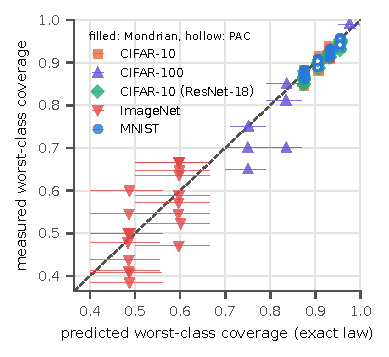
\includegraphics[width=.3\linewidth]{worst_class_theory.pdf}\hfill
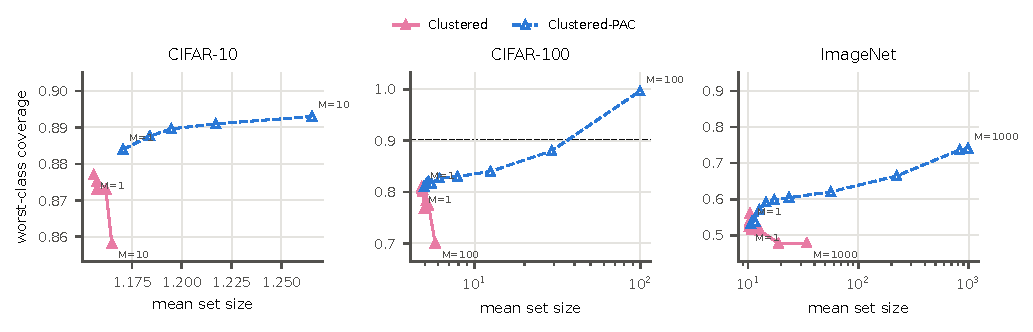
\includegraphics[width=.68\linewidth]{clusters_main.pdf}
\caption{Left: measured vs predicted worst-class coverage (Prop.~1), every run, seed and $\alpha$; filled Mondrian, hollow PAC.
Right: cluster count $M$ from 1 (marginal) to $K$, size vs worst class, without (solid) and with (dashed) the PAC correction. At $M{=}K$, $k$-means still merges a few classes, so the dashed end point is not Mondrian-PAC.}
\label{fig:main}
\end{figure}
\textbf{Validity.} Every method with an on-average guarantee covers \CovLo--\CovHi\% at $\alpha=0.1$ (Table~\ref{tab:main}). The PAC versions
cover more, as they should.
\textbf{Who is left out.} Naive($T$), the smallest-set score, covers its worst class \WorstCTenNaiveT\% of the time on CIFAR-10,
\WorstCHunNaiveT\% on CIFAR-100 and \WorstINetNaiveT\% on ImageNet. That gap is large. On CIFAR-10 the worst class is \ErrCTenCls\
(\ErrCTenCov\%), and \ErrCTenConfShare\% of its misclassified images are called \ErrCTenConf. The worst cluster of test features fares no
better (\FscCTenNaiveT\%). APS($T$) buys balance with bigger sets: its worst class is \WorstCTenAPST, \WorstCHunAPST\ and
\WorstINetAPST\%. MNIST shows a different failure. Accuracy is above $1-\alpha$, so the method can only hit the target by leaving
\EmptyMNISTNaive\% of sets empty.
\textbf{Per-class calibration is not enough.} Mondrian protects each class only on average over calibration draws. With about 20
images per class, its worst ImageNet class is \WorstINetMond\% at \SizeINetMond\ labels.
\textbf{Repair.} Mondrian-PAC lifts CIFAR-10's worst class to \WorstCTenMondPAC\% at size \SizeCTenMondPAC\ (bootstrap gain
+\BsCTenPacVsMondW\ points, CI [\BsCTenPacVsMondWLo, \BsCTenPacVsMondWHi]). On ImageNet it can't work at all and returns every label.
Clustered-PAC reaches \WorstINetClusPAC\% with \SizeINetClusPAC\ labels, which beats Mondrian on both counts. On CIFAR-100 it reaches
\WorstCHunClusPAC\% at \SizeCHunClusPAC\ labels, where Mondrian-PAC needs \SizeCHunMondPAC\ (Figure~\ref{fig:main}).
\textbf{Weak results.} My first idea, the distance term, adds only \BsCTenDistVsNaiveW\ points to CIFAR-10's worst class (CI
[\BsCTenDistVsNaiveWLo, \BsCTenDistVsNaiveWHi]). APS($T$) does far better, and on CIFAR-100 the distance term does nothing
(\WorstCHunDist\ vs \WorstCHunNaiveT\%). The learned score doesn't shrink sets (\SizeCTenLearned\ vs \SizeCTenNaiveT) and lowers the
worst class. The pretrained ResNet-18 tells the same story: its worst class is \WorstCTenRNaiveT, \WorstCTenRAPST, \WorstCTenRClusPAC\
and \WorstCTenRMondPAC\% for Naive($T$), APS($T$), Clustered-PAC and Mondrian-PAC.
\textbf{In short:} every method keeps its average promise, but its worst class can fall below half, and only grouped
high-probability cut-offs fix that cheaply.

\section{Theory and Failure Audit}\label{sec:depth}
\textbf{Derivation.} If the test image is exchangeable with the calibration images (drawn from the same source) and scores never tie,
its score is equally likely to take any rank among the $n{+}1$ scores. So $P(Y\in C)=k/(n{+}1)\in[1-\alpha,1-\alpha+\tfrac1{n+1})$. For one fixed $D_\text{cal}$, coverage is
$F(S_{(k)})\sim\mathrm{Beta}(k,n{+}1{-}k)$ \citep{angelopoulos2021gentle}. At $n=100$, \BelowHundred\% of 200 re-splits land below
$1-\alpha$.
\textbf{Proposition 1 (worst-class law).} With per-class cut-offs, each class is calibrated on its own images. Their coverages
are therefore independent, each $\mathrm{Beta}(k_c,n_c{+}1{-}k_c)$, and Beta--binomial when measured on $m_c$ test images. Hence
$P(\min_c\widehat{\mathrm{cov}}_c\ge t)=\prod_cP(\widehat{\mathrm{cov}}_c\ge t)$. Intuitively, the worst class is the unluckiest of $K$
independent draws: more classes or fewer images per class push it lower. Predicted and measured Mondrian worst class: CIFAR-10
\PredCTenMond/\MeasCTenMond, CIFAR-100 \PredCHunMond/\MeasCHunMond, ImageNet \PredINetMond/\MeasINetMond\%. On random re-splits of the calibration
and test images, where the assumption holds by design, the law is within \NsMaxErr\ points everywhere. CIFAR-100's official test set sits \MissPtsCHun\
points below it (Fisher $p=\FisherCHun$ over seeds). I read this as the per-class train/test shift that \citet{recht2018cifar} report,
and the law catches it. To keep every class within 2 points with probability 0.9, you need \NeedTen, \NeedHun\ and \NeedThou\ images
per class for $K=10$, 100 and 1000. The same independence makes the PAC level $\delta_g$ exact (no union bound is needed). It also sets a
floor: a finite threshold needs $n_g\ge\lceil\log\delta_g/\log(1-\alpha)\rceil$, which is \PacMinINet\ on ImageNet.
\textbf{Overall $\ne$ per class, and label shift.} Coverage is $\sum_c\pi_c\mathrm{cov}_c$. If the mix of classes changes to $\pi'$, it can
fall all the way to $\min_c\mathrm{cov}_c$. When I randomly and strongly change the class mix on CIFAR-10, Naive($T$)'s worst draw is
\LsCTenNaiveMin\%, while Mondrian-PAC's is \LsCTenMondPACMin\%. A guarantee for every single image is impossible unless the sets are uselessly large
\citep{vovk2012conditional,barber2021limits}.
\textbf{Failure audit.} On CIFAR-10.1, APS($T$) covers \TenCTenAPST\%. At CIFAR-10-C severity 5 it drops to \CcCTenAPSTSFive\%. On a
stream that drifts into corruption, ACI lifts the worst segment from \AciCTenFixCov\% to \AciCTenAciCov\%, by growing sets from
\AciCTenFixSize\ to \AciCTenAciSize\ labels. Covariate-shift weighting lifts coverage from \WtCovStdCTen\% to \WtCovWCTen\%, but only
by returning every label for \WtInfCTen\% of images: shifted and clean images barely overlap. As for the distance score, it helps little
because the softmax already ranks the deciding second label better (AUROC \DdSoftCTen\ vs \DdDistCTen).

\section{Limitations and Conclusion}
The worst-class law covers per-class calibration and assumes each class's test images look like its calibration images.
Clustered-PAC protects clusters, not single classes, and its clusters come from a small design split. The ImageNet seeds re-split one
model's outputs, and my shifts are synthetic or benchmark corruptions, not a real deployment.
\textbf{Conclusion.} The score decides who gets covered. The grouping decides which classes are protected. The worst class can be
predicted before deployment from the class counts alone. Guaranteeing it class by class takes thousands of images per class, but
sharing corrected thresholds across similar classes protects it with high probability at a fraction of that cost (\SizeINetClusPAC\
labels per set on ImageNet, not 1{,}000). I think papers should report the worst class and the empty-set rate next to marginal coverage.

\section{Reproducibility and AI-Use Disclosure}
The scripts in \texttt{scripts/} train every model and regenerate every table, figure and number; \texttt{paper\_numbers.py} writes
the numbers as macros, so none is typed by hand, and \texttt{pytest tests/} runs 22 checks. Seeds, splits and settings are in
\texttt{configs/default.yaml}. The site \texttt{sumitjhaa.github.io/conformal-worst-class} re-runs conformal prediction in the browser.
AI assistance (Claude) helped organise the code, build parts of the interactive site and explorers, and edit the report's wording and
structure. The experiments, analysis and results are my own.

{\small\setlength{\bibsep}{0.8pt}
\bibliographystyle{unsrtnat}
\bibliography{refs}}

\end{document}
